\chapter{Multimedia Chat mit Firebase ->Putz}
\putz

\section{EMS Chat}
Bei EMS war bei beginn des Projektes eine integrierte Chatfunktion geplant. Ein Promoter sollte, bei eventuellen Fragen zum Event einen Administrator/Eventmanager um Hilfe bitten können. Ein Administrator sollte mit bestimmten
Promotern gezielt einen Chat starten können, sowie auch an alle Promoter eines Events eine Sammelnachricht senden können. Promoter untereinander sollten aus Datenschutzrechtlichen gründen, aber vor allem auch in erster
Linie vor Konkurrenzschutz, nicht chatten können.
Es wurde über drei Sprints hinweg versucht einen eigenständigen Chat in der EMS Software zu integrieren. Dies gelang schlussendlich mit dem zuletzt versuchten Lösungsansatz nicht.
Es hat erhebliche Probleme mit den \textbf{CORS Policys} auf Seiten des Backends gegeben. Im Frontend in Ionic/Angular war der Chat fertig implementiert. Der Chat basierte auf einer Lösung dem npm package \textbf{socket.io}\footcite{socket-io}.


Mehrer Ansätze zum lösen des Fehlers, auch mit Einbezug externer Personen sowie des Betreuers blieben erfolglos. Auch eine temporäre, sicherheitstechnisch undenkbare Methode, nämlich alle Aktivitäten zu erlauben, wie im untenstehenden Beispielcode beschrieben, führte zu keinem Erfolg.

\begin{lstlisting}[language=bash]
#app ist die express instanz
#app nutzt cors und erlaubt sämtliche requests auf den server 

app.use(cors());

app.all('/', function(req, res, next) {
  res.header("Access-Control-Allow-Origin", "*");
  res.header("Access-Control-Allow-Headers", "Origin, X-Requested-With, Content-Type, Accept");
  next()
});
\end{lstlisting}

Stattdessen wurde die Funktion auf einen Patch nach dem eigentlichen Release verschoben und parallel mit der Entwicklung einer eigenständigen Chatapplikation, welche einen neuen Ansatz verfolgt, begonnen. Stand zur Verfassung des Dokumentes ist diese eigenständige Version
voll lauffähig und wird in die EMS Applikation im nachhinein integriert werden. In einem Gespräch innerhalb der Gruppe, wurde das Fazit bezüglich dieser User-Story gezogen, dass in Zukunft bei einer Story, welche nach zwei Mal verschieben noch immer nicht
fertig wurde, sollte diese nicht eine Hauptkomponente sein, einem internen Review unterzogen wird um alternativen für die Implementierung zu finden.

\subsection{Firebase Chatapp}
Um eine Chatapp\footcite{Chatapp-Beispiel} mithilfe des Firebase Modules zu erstellen, benötigt man zuerst ein Konto auf der Firebase Homepage, zu erstellen unter der offiziellen Webseite\footcite{firebase-site} des Anbieter.
Nachdem dies erledigt wurde wechselt man auf seine Konsole und erstellt ein neuen Projekt. Man kann das neue Projekt auch direkt einer in Besitz befindenden Domain. Nach Erstellung eines neuen Projekts landet man aus der Übersichtsseite
von diesem (Abb. 3.1).

\begin{center}
    \begin{figure}[h]
        \centering
        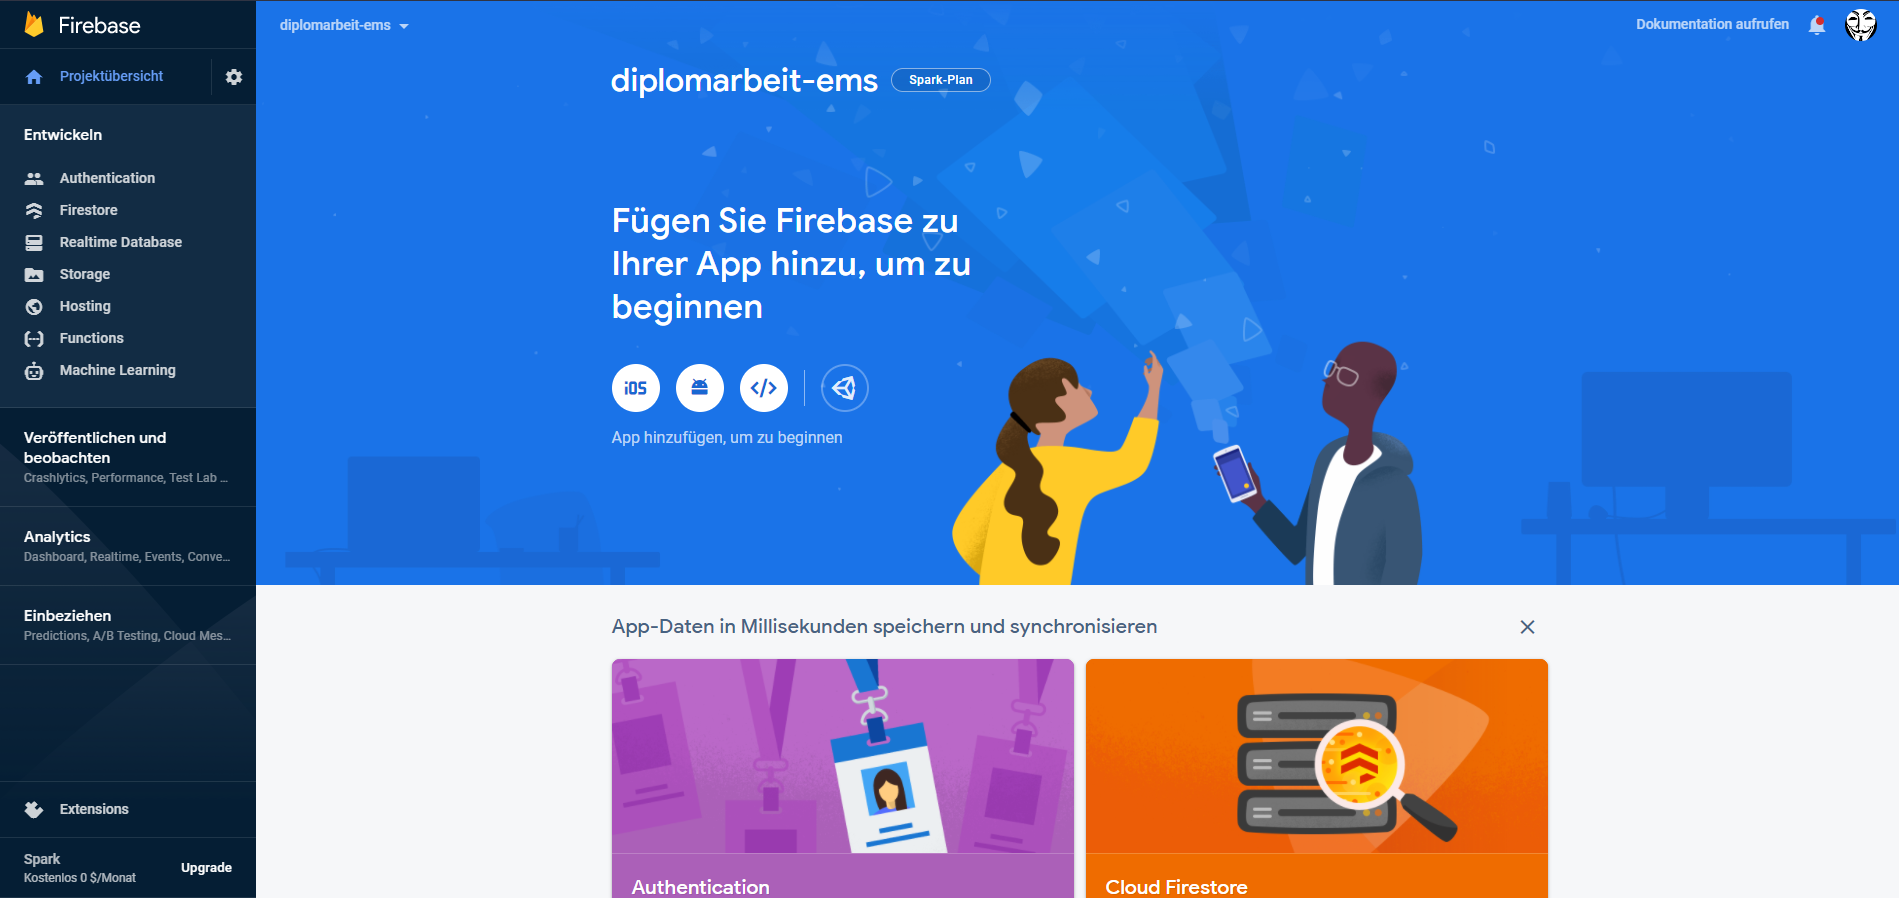
\includegraphics[width=\textwidth]{firebase-main.png}
        \caption{Datenbank erstellen}
    \end{figure}
\end{center}

Nachdem man auf der linken Seite auf "`Realtime Database"' geklickt hat, lädt die Hauptkomponente der Seite neu, nun klickt man auf Datenbank erstellen (Abb. 3.2).

\begin{center}
    \begin{figure}[h]
        \centering
        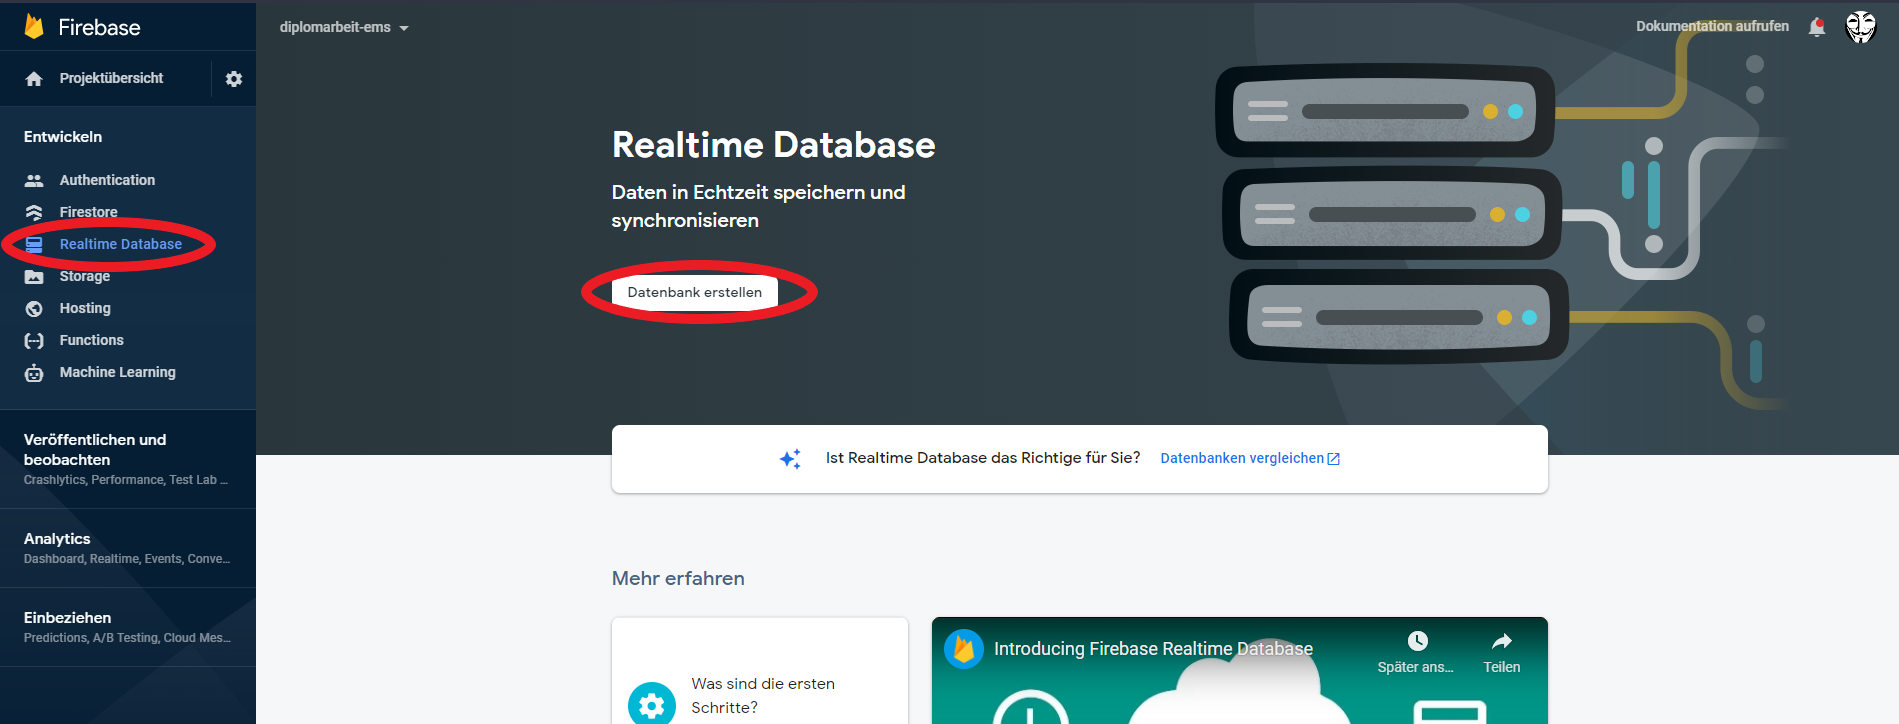
\includegraphics[width=\textwidth]{firebase-db1.png}
        \caption{Datenbank erstellen}
    \end{figure}
\end{center}

Danach erscheint ein Pop-up in welchem man der Ort, wo die Daten der Datenbank gespeichert werden, festgelegt werden. Da die Software DSGVO konform sein muss, sollte ein einen Standort innerhalb der EU aus.

\begin{center}
    \begin{figure}[h]
        \centering
        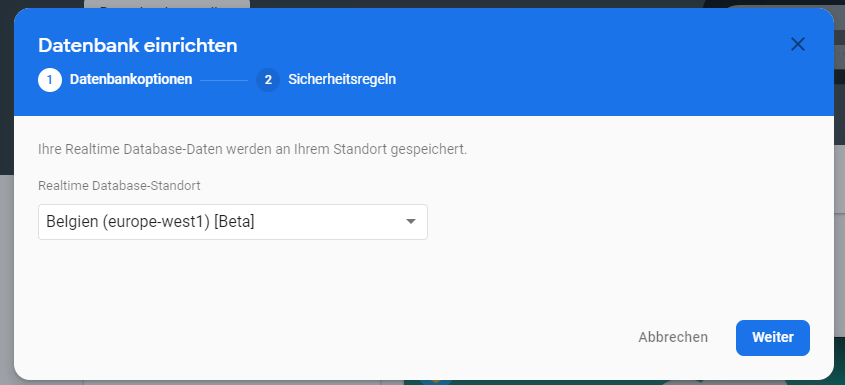
\includegraphics[width=\textwidth]{firebase-db2.png}
        \caption{Datenbank Standort}
    \end{figure}
\end{center}

Mit einem Klick auf Weiter, gelangt man auf die zweite und letzte Seite des Pop-ups. Hier kann man nun auswählen ob die Datenbank direkt in Produktivbetrieb geht oder zuerst der Testmodus gestartet werden soll. Dies ist bei einer
noch aktiven Entwicklung zu empfehlen wie auf den Hinweisen in Abb. 3.3 zu lesen ist.

\begin{center}
    \begin{figure}[h]
        \centering
        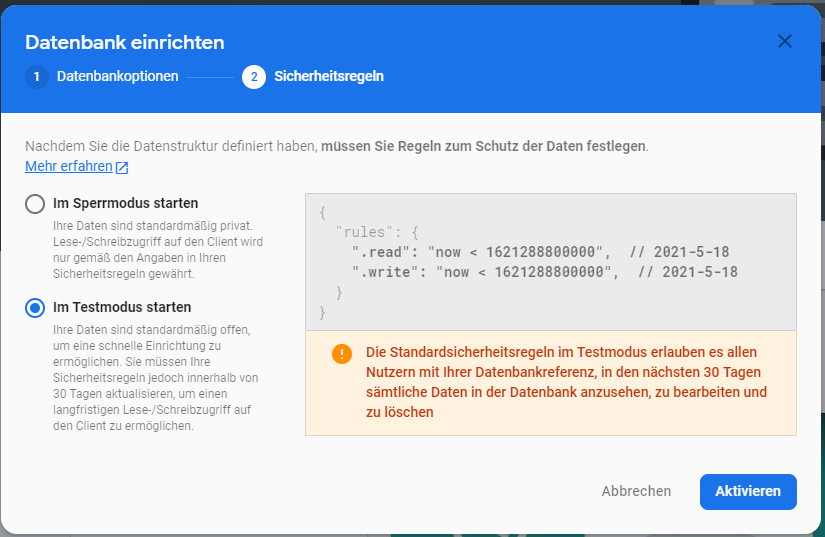
\includegraphics[width=\textwidth]{firebase-db3.png}
        \caption{Datenbank Modus}
    \end{figure}
\end{center}

Nun wurde eine fertige Realtime Database in Firebase erstellt. Damit die nachfolgende Angular App auch mit der Datenbank kommunizieren kann, müssen nur für jetzt zum testen im Testmodus, die Lese- und Schreibrechte auf
jeden übertragen werden. Dies ist in Abb. 3.4 zu sehen.

\begin{center}
    \begin{figure}[h]
        \centering
        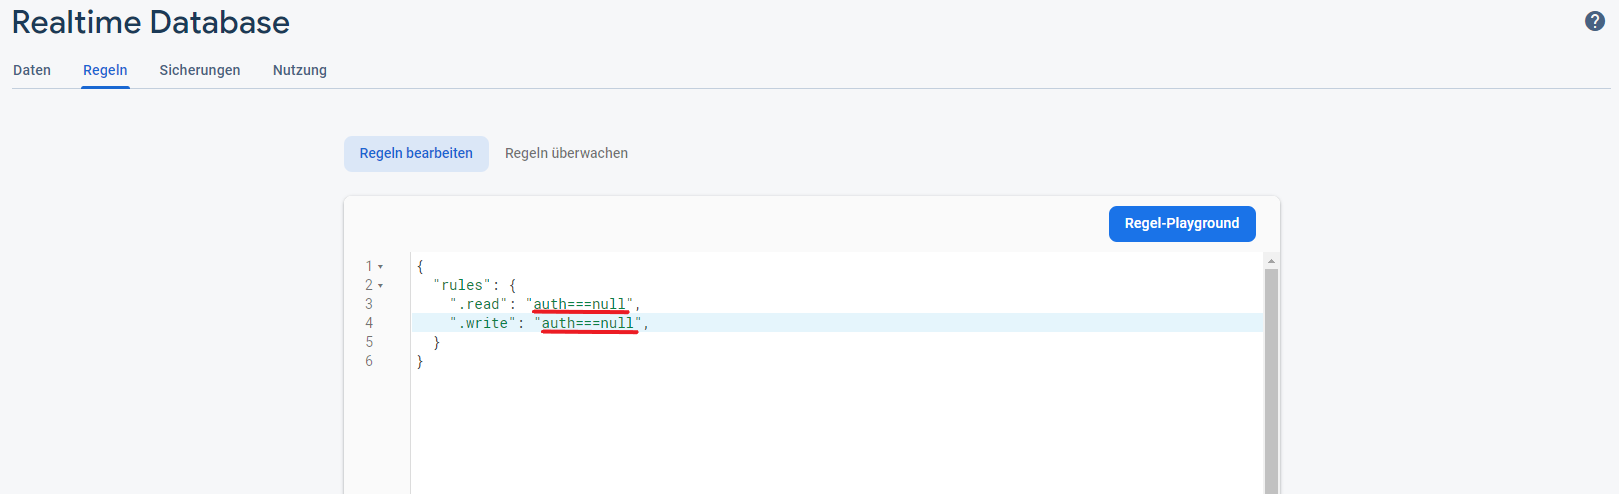
\includegraphics[width=\textwidth]{firebase-db4.png}
        \caption{Datenbank Regeln bearbeiten}
    \end{figure}
\end{center}

Dies war die Konfiguration der Datenbank hinter der Chatapplilation in der Firebase Cloud. Nun folgt eine Anleitung und einige Codesnippets zu Erstellung des eigentlich Chatprogrammes in Angular, welches später in das Hauptprogramm
EMS integriert wird.

Zuerst muss das Google Firebase SDK installiert und auch in einer neuen Angular App inkludiert werden.

\begin{lstlisting}[language=bash]
    #Installieren
    npm install --save firebase

    #In Datei `src/app/app.component.ts` vom Home Verzeichnis 
    #des Projektes aus importieren
    import * as firebase from 'firebase';
\end{lstlisting}

Als nächstes wurden der API Key und die URL zur Datenbank in Firebase gesetzt.



%da war ich https://www.djamware.com/post/5ee1d127711dcf4b441296de/angular-9-tutorial-creating-firebase-chat-web-app#setup-firebase


\newpage